%---------------
%╔═╗╔═╗╔╦╗╦  ╦╔═╗
%╚═╗║╣    ║  ║  ║╠═╝
%╚═╝╚═╝  ╩  ╚═╝╩  
%---------------

% language setup
\newcommand{\docLanguage}{ngerman}
%\newcommand{\docLanguage}{english}

% DOCUMENT SETUP
\documentclass[12pt, oneside, a4paper, \docLanguage]{report}
\usepackage[left=3cm, 
			right=2.5cm, 
			top=2.5cm, 
			bottom=2.5cm, 
			includehead, 
			includefoot]{geometry}

% line spacing
\usepackage{setspace}
\setstretch{1,25} % 15/12 --> 1.25

% encoding setup
% T1 font encoding for languages that use a latin alphabet
\usepackage[T1]{fontenc} 

% enhanced input encoding handling - utf8 for äÄüÜöÖß...
\usepackage[utf8]{inputenc}

%de­fines Adobe Times Ro­man as de­fault text font
\usepackage{mathptmx}
\usepackage{times} % needed for acronym package

%PDF linking package
\usepackage[hidelinks]{hyperref}


% Language Setup
\usepackage[\docLanguage]{babel}
% after babel - set chapter string
\AtBeginDocument{\renewcommand{\chaptername}{}}

% language specific bibliography style
\usepackage[numbers, square]{natbib}
%\setcitestyle{square,aysep={},yysep={;}}
\usepackage[fixlanguage]{babelbib}
\selectbiblanguage{\docLanguage}
% bliographystyle setup
% babel specific: babplain, babplai3, babalpha, babunsrt, bababbrv, bababbr3
\bibliographystyle{babunsrt}


% enumeration
\usepackage{enumitem}
% tabular extension tabularx
\usepackage{tabularx}

% math packages
\usepackage{amsmath}
\usepackage{nicefrac}
\usepackage{amsthm}
\usepackage{amsbsy}
\usepackage{amssymb}
\usepackage{amsfonts}
%\usepackage{MnSymbol}


%special characters
\usepackage{amssymb}
\usepackage{upgreek,textgreek}

% acronym package
\usepackage[printonlyused, footnote]{acronym}

% breakable text in \seqsplit{}
\usepackage{seqsplit}

% \textmu
\usepackage{textcomp}

% package provides a way to compile sections of a document using the same preamble as the main document
\usepackage{subfiles}

% driver-independent color extension - used by listings,tabularx
\usepackage[usenames,dvipsnames,table,xcdraw]{xcolor}

% -- SYNTAX HIGHLIGHTING --
\usepackage{listings}
%% bash command line Syntax Highlighting
\lstdefinestyle{BASH_CMD}{ 
  columns=fullflexible,            % copy pasteable listings
  language=bash,
  basicstyle=\small\sffamily,
  basicstyle   = \small \ttfamily,
  keywordstyle = [1]\small \ttfamily,
  keywordstyle = [2]\small \ttfamily,
  commentstyle = \small \ttfamily,
  numbers=none,
  captionpos=b, 
  breaklines=true,
  numberstyle=\tiny,
  numbersep=3pt,
  frame=tlrb,
  columns=fullflexible,
  backgroundcolor=\color{white!20},
  linewidth=\linewidth,
  literate=                        % replace in code
     {Ö}{{\"O}}1 
     {Ä}{{\"A}}1 
     {Ü}{{\"U}}1 
     {ß}{{\ss}}2 
     {ü}{{\"u}}1 
     {ä}{{\"a}}1 
     {ö}{{\"o}}1 
     {â}{{\^{a}}}1 
     {Â}{{\^{A}}}1 
     {ç}{{\c{c}}}1 
     {Ç}{{\c{C}}}1 
     {ğ}{{\u{g}}}1 
     {Ğ}{{\u{G}}}1 
     {ı}{{\i}}1 
     {İ}{{\.{I}}}1 
     {ş}{{\c{s}}}1 
     {Ş}{{\c{S}}}1 
}
 % adds style BASH_CMD
%% Matlab Syntax Highlighting
\colorlet{keyword}{blue!100!black!80}
\colorlet{STD}{Lavender}
\colorlet{comment}{green!90!black!90}
\definecolor{mygreen}{rgb}{0,0.6,0}
\definecolor{mygray}{rgb}{0.5,0.5,0.5}
\definecolor{mymauve}{rgb}{0.58,0,0.82}


\lstdefinestyle{BASH_SCRIPT}{ 
  language     = bash,
  basicstyle   = \footnotesize \ttfamily,
  keywordstyle = [1]\color{keyword}\bfseries,
  keywordstyle = [2]\color{STD}\bfseries,
  commentstyle = \color{mygreen}\itshape,
  backgroundcolor=\color{white},   % choose the background color; you must add \usepackage{color} 
  columns=fullflexible,            % copy pasteable listings
                                   % or \usepackage{xcolor}
  basicstyle=\footnotesize,        % the size of the fonts that are used for the code
  breakatwhitespace=false,         % sets if automatic breaks should only happen at whitespace
  breaklines=true,                 % sets automatic line breaking
  captionpos=b,                    % sets the caption-position to bottom
  extendedchars=true,              % lets you use non-ASCII characters; for 8-bits encodings only,
                                   % does not work with UTF-8
  frame=single,                    % adds a frame around the code
  keepspaces=true,                 % keeps spaces in text, useful for keeping indentation of code
                                   % (possibly needs columns=flexible)
  numbers=left,                    % where to put the line-numbers; possible values are 
                                   % (none, left, right)
  numbersep=5pt,                   % how far the line-numbers are from the code
  numberstyle=\tiny\color{mygray}, % the style that is used for the line-numbers
  rulecolor=\color{black},         % if not set, the frame-color may be changed on line-breaks
                                   % within not-black text (e.g. comments (green here))
  showspaces=false,                % show spaces everywhere adding particular underscores; it
  	                               % overrides 'showstringspaces'
  showstringspaces=false,          % underline spaces within strings only
  showtabs=false,                  % show tabs within strings adding particular underscores
  stepnumber=1,                    % the step between two line-numbers. If it's 1, each line 
                                   % will be numbered
  stringstyle=\color{mymauve},     % string literal style
  tabsize=2,                       % sets default tabsize to 2 spaces
  title=\lstname,                  % set title name
  literate=                        % replace in code
     {Ö}{{\"O}}1 
     {Ä}{{\"A}}1 
     {Ü}{{\"U}}1 
     {ß}{{\ss}}2 
     {ü}{{\"u}}1 
     {ä}{{\"a}}1 
     {ö}{{\"o}}1 
     {â}{{\^{a}}}1 
     {Â}{{\^{A}}}1 
     {ç}{{\c{c}}}1 
     {Ç}{{\c{C}}}1 
     {ğ}{{\u{g}}}1 
     {Ğ}{{\u{G}}}1 
     {ı}{{\i}}1 
     {İ}{{\.{I}}}1 
     {ş}{{\c{s}}}1 
     {Ş}{{\c{S}}}1 
} % adds style BASH_SCRIPT
% Matlab Syntax Highlighting
\colorlet{keyword}{blue!100!black!80}
\colorlet{STD}{red}
\colorlet{comment}{green!90!black!90}
\definecolor{mygreen}{rgb}{0,0.6,0}
\definecolor{mygray}{rgb}{0.5,0.5,0.5}
\definecolor{mymauve}{rgb}{0.58,0,0.82}


\lstdefinestyle{LATEX}{ 
  language     = [LaTeX]{TeX},
  basicstyle   = \footnotesize \ttfamily,
  keywordstyle = [1]\color{keyword}\bfseries,
  keywordstyle = [2]\color{comment}\bfseries,
  commentstyle = \color{mygray}\itshape,
  %backgroundcolor=\color{white},   % choose the background color; you must add \usepackage{color} 
                                   % or \usepackage{xcolor}
  basicstyle=\footnotesize,        		   % the size of the fonts that are used for the code
  breakatwhitespace=false,         % sets if automatic breaks should only happen at whitespace
  columns=fullflexible,            % copy pasteable listings
  breaklines=true,                 % sets automatic line breaking
  captionpos=c,                    % sets the caption-position to bottom
  extendedchars=true,              % lets you use non-ASCII characters; for 8-bits encodings only,
                                   % does not work with UTF-8
  frame=single,                    % adds a frame around the code
  keepspaces=true,                 % keeps spaces in text, useful for keeping indentation of code
                                   % (possibly needs columns=flexible)
  numbers=left,                    % where to put the line-numbers; possible values are 
                                   % (none, left, right)
  numbersep=4pt,                   % how far the line-numbers are from the code
  numberstyle=\tiny\color{mygray}, % the style that is used for the line-numbers
  rulecolor=\color{black},         % if not set, the frame-color may be changed on line-breaks
                                   % within not-black text (e.g. comments (green here))
  showspaces=false,                % show spaces everywhere adding particular underscores; it
  	                               % overrides 'showstringspaces'
  showstringspaces=false,          % underline spaces within strings only
  showtabs=false,                  % show tabs within strings adding particular underscores
  stepnumber=1,                    % the step between two line-numbers. If it's 1, each line 
                                   % will be numbered
  stringstyle=\color{mymauve},     % string literal style
  tabsize=2,                       % sets default tabsize to 2 spaces
  title=\lstname,                  % set title name
  literate=                        % replace in code
     {Ö}{{\"O}}1 
     {Ä}{{\"A}}1 
     {Ü}{{\"U}}1 
     {ß}{{\ss}}2 
     {ü}{{\"u}}1 
     {ä}{{\"a}}1 
     {ö}{{\"o}}1 
     {â}{{\^{a}}}1 
     {Â}{{\^{A}}}1 
     {ç}{{\c{c}}}1 
     {Ç}{{\c{C}}}1 
     {ğ}{{\u{g}}}1 
     {Ğ}{{\u{G}}}1 
     {ı}{{\i}}1 
     {İ}{{\.{I}}}1 
     {ş}{{\c{s}}}1 
     {Ş}{{\c{S}}}1 
} % adds style LATEX
%% Matlab Syntax Highlighting
\colorlet{keyword}{blue!100!black!80}
\colorlet{STD}{Lavender}
\colorlet{comment}{green!90!black!90}
\definecolor{mygreen}{rgb}{0,0.6,0}
\definecolor{mygray}{rgb}{0.5,0.5,0.5}
\definecolor{mymauve}{rgb}{0.58,0,0.82}


\lstdefinestyle{MATLAB}{ 
  language     = Matlab,
  basicstyle   = \footnotesize \ttfamily,
  keywordstyle = [1]\color{keyword}\bfseries,
  keywordstyle = [2]\color{STD}\bfseries,
  commentstyle = \color{mygreen}\itshape,
  backgroundcolor=\color{white},   % choose the background color; you must add \usepackage{color} 
                                   % or \usepackage{xcolor}
  basicstyle=\footnotesize,        % the size of the fonts that are used for the code
  breakatwhitespace=false,         % sets if automatic breaks should only happen at whitespace
  columns=fullflexible,            % copy pasteable listings
  breaklines=false,                % sets automatic line breaking
  captionpos=c,                    % sets the caption-position to bottom
  extendedchars=true,              % lets you use non-ASCII characters; for 8-bits encodings only,
                                   % does not work with UTF-8
  frame=single,                    % adds a frame around the code
  keepspaces=true,                 % keeps spaces in text, useful for keeping indentation of code
                                   % (possibly needs columns=flexible)
  numbers=left,                    % where to put the line-numbers; possible values are 
                                   % (none, left, right)
  numbersep=5pt,                   % how far the line-numbers are from the code
  numberstyle=\tiny\color{mygray}, % the style that is used for the line-numbers
  rulecolor=\color{black},         % if not set, the frame-color may be changed on line-breaks
                                   % within not-black text (e.g. comments (green here))
  showspaces=false,                % show spaces everywhere adding particular underscores; it
  	                               % overrides 'showstringspaces'
  showstringspaces=false,          % underline spaces within strings only
  showtabs=false,                  % show tabs within strings adding particular underscores
  stepnumber=1,                    % the step between two line-numbers. If it's 1, each line 
                                   % will be numbered
  stringstyle=\color{mymauve},     % string literal style
  tabsize=2,                       % sets default tabsize to 2 spaces
  title=\lstname,                  % set title name
  literate=                        % replace in code
     {Ö}{{\"O}}1 
     {Ä}{{\"A}}1 
     {Ü}{{\"U}}1 
     {ß}{{\ss}}2 
     {ü}{{\"u}}1 
     {ä}{{\"a}}1 
     {ö}{{\"o}}1 
     {â}{{\^{a}}}1 
     {Â}{{\^{A}}}1 
     {ç}{{\c{c}}}1 
     {Ç}{{\c{C}}}1 
     {ğ}{{\u{g}}}1 
     {Ğ}{{\u{G}}}1 
     {ı}{{\i}}1 
     {İ}{{\.{I}}}1 
     {ş}{{\c{s}}}1 
     {Ş}{{\c{S}}}1 
} % adds style MATLAB
% Matlab Syntax Highlighting
\colorlet{keyword}{blue!100!black!80}
\colorlet{STD}{Lavender}
\colorlet{comment}{green!90!black!90}
\definecolor{mygreen}{rgb}{0,0.6,0}
\definecolor{mygray}{rgb}{0.5,0.5,0.5}
\definecolor{mymauve}{rgb}{0.58,0,0.82}


\lstdefinestyle{PYTHON}{ 
  language     = Python,
  basicstyle   = \footnotesize \ttfamily,
  keywordstyle = [1]\color{keyword}\bfseries,
  keywordstyle = [2]\color{STD}\bfseries,
  commentstyle = \color{mygreen}\itshape,
  backgroundcolor=\color{white},   % choose the background color; you must add \usepackage{color} 
                                   % or \usepackage{xcolor}
  basicstyle=\footnotesize,        % the size of the fonts that are used for the code
  columns=fullflexible,            % copy pasteable listings
  breakatwhitespace=false,         % sets if automatic breaks should only happen at whitespace
  breaklines=false,                % sets automatic line breaking
  captionpos=c,                    % sets the caption-position to bottom
  extendedchars=true,              % lets you use non-ASCII characters; for 8-bits encodings only,
                                   % does not work with UTF-8
  frame=single,                    % adds a frame around the code
  keepspaces=true,                 % keeps spaces in text, useful for keeping indentation of code
                                   % (possibly needs columns=flexible)
  numbers=left,                    % where to put the line-numbers; possible values are 
                                   % (none, left, right)
  numbersep=5pt,                   % how far the line-numbers are from the code
  numberstyle=\tiny\color{mygray}, % the style that is used for the line-numbers
  rulecolor=\color{black},         % if not set, the frame-color may be changed on line-breaks
                                   % within not-black text (e.g. comments (green here))
  showspaces=false,                % show spaces everywhere adding particular underscores; it
  	                               % overrides 'showstringspaces'
  showstringspaces=false,          % underline spaces within strings only
  showtabs=false,                  % show tabs within strings adding particular underscores
  stepnumber=1,                    % the step between two line-numbers. If it's 1, each line 
                                   % will be numbered
  stringstyle=\color{mymauve},     % string literal style
  tabsize=2,                       % sets default tabsize to 2 spaces
  title=\lstname,                  % set title name
  literate=                        % replace in code
     {Ö}{{\"O}}1 
     {Ä}{{\"A}}1 
     {Ü}{{\"U}}1 
     {ß}{{\ss}}2 
     {ü}{{\"u}}1 
     {ä}{{\"a}}1 
     {ö}{{\"o}}1 
     {â}{{\^{a}}}1 
     {Â}{{\^{A}}}1 
     {ç}{{\c{c}}}1 
     {Ç}{{\c{C}}}1 
     {ğ}{{\u{g}}}1 
     {Ğ}{{\u{G}}}1 
     {ı}{{\i}}1 
     {İ}{{\.{I}}}1 
     {ş}{{\c{s}}}1 
     {Ş}{{\c{S}}}1 
} % adds style PYTHON
%% Matlab Syntax Highlighting
\colorlet{keyword}{blue!100!black!80}
\colorlet{STD}{Lavender}
\colorlet{comment}{green!90!black!90}
\definecolor{mygreen}{rgb}{0,0.6,0}
\definecolor{mygray}{rgb}{0.5,0.5,0.5}
\definecolor{mymauve}{rgb}{0.58,0,0.82}


\lstdefinestyle{CPP}{ 
  language     = C++,
  basicstyle   = \footnotesize \ttfamily,
  keywordstyle = [1]\color{keyword}\bfseries,
  keywordstyle = [2]\color{STD}\bfseries,
  commentstyle = \color{mygreen}\itshape,
  backgroundcolor=\color{white},   % choose the background color; you must add \usepackage{color} 
                                   % or \usepackage{xcolor}
  columns=fullflexible,            % copy pasteable listings
  basicstyle=\footnotesize,        % the size of the fonts that are used for the code
  breakatwhitespace=false,         % sets if automatic breaks should only happen at whitespace
  breaklines=false,                % sets automatic line breaking
  captionpos=c,                    % sets the caption-position to bottom
  extendedchars=true,              % lets you use non-ASCII characters; for 8-bits encodings only,
                                   % does not work with UTF-8
  frame=single,                    % adds a frame around the code
  keepspaces=true,                 % keeps spaces in text, useful for keeping indentation of code
                                   % (possibly needs columns=flexible)
  numbers=left,                    % where to put the line-numbers; possible values are 
                                   % (none, left, right)
  numbersep=5pt,                   % how far the line-numbers are from the code
  numberstyle=\tiny\color{mygray}, % the style that is used for the line-numbers
  rulecolor=\color{black},         % if not set, the frame-color may be changed on line-breaks
                                   % within not-black text (e.g. comments (green here))
  showspaces=false,                % show spaces everywhere adding particular underscores; it
  	                               % overrides 'showstringspaces'
  showstringspaces=false,          % underline spaces within strings only
  showtabs=false,                  % show tabs within strings adding particular underscores
  stepnumber=1,                    % the step between two line-numbers. If it's 1, each line 
                                   % will be numbered
  stringstyle=\color{mymauve},     % string literal style
  tabsize=2,                       % sets default tabsize to 2 spaces
  title=\lstname,                  % set title name
  literate=                        % replace in code
     {Ö}{{\"O}}1 
     {Ä}{{\"A}}1 
     {Ü}{{\"U}}1 
     {ß}{{\ss}}2 
     {ü}{{\"u}}1 
     {ä}{{\"a}}1 
     {ö}{{\"o}}1 
     {â}{{\^{a}}}1 
     {Â}{{\^{A}}}1 
     {ç}{{\c{c}}}1 
     {Ç}{{\c{C}}}1 
     {ğ}{{\u{g}}}1 
     {Ğ}{{\u{G}}}1 
     {ı}{{\i}}1 
     {İ}{{\.{I}}}1 
     {ş}{{\c{s}}}1 
     {Ş}{{\c{S}}}1 
} % adds style CPP
%% Matlab Syntax Highlighting
\colorlet{keyword}{blue!100!black!80}
\colorlet{STD}{Lavender}
\colorlet{comment}{green!90!black!90}
\definecolor{mygreen}{rgb}{0,0.6,0}
\definecolor{mygray}{rgb}{0.5,0.5,0.5}
\definecolor{mymauve}{rgb}{0.58,0,0.82}


\lstdefinestyle{C}{ 
  language     = C,
  basicstyle   = \footnotesize \ttfamily,
  keywordstyle = [1]\color{keyword}\bfseries,
  keywordstyle = [2]\color{STD}\bfseries,
  commentstyle = \color{mygreen}\itshape,
  backgroundcolor=\color{white},   % choose the background color; you must add \usepackage{color} 
  columns=fullflexible,            % copy pasteable listings
                                   % or \usepackage{xcolor}
  basicstyle=\footnotesize,        % the size of the fonts that are used for the code
  breakatwhitespace=false,         % sets if automatic breaks should only happen at whitespace
  breaklines=false,                % sets automatic line breaking
  captionpos=c,                    % sets the caption-position to bottom
  extendedchars=true,              % lets you use non-ASCII characters; for 8-bits encodings only,
                                   % does not work with UTF-8
  frame=single,                    % adds a frame around the code
  keepspaces=true,                 % keeps spaces in text, useful for keeping indentation of code
                                   % (possibly needs columns=flexible)
  numbers=left,                    % where to put the line-numbers; possible values are 
                                   % (none, left, right)
  numbersep=5pt,                   % how far the line-numbers are from the code
  numberstyle=\tiny\color{mygray}, % the style that is used for the line-numbers
  rulecolor=\color{black},         % if not set, the frame-color may be changed on line-breaks
                                   % within not-black text (e.g. comments (green here))
  showspaces=false,                % show spaces everywhere adding particular underscores; it
  	                               % overrides 'showstringspaces'
  showstringspaces=false,          % underline spaces within strings only
  showtabs=false,                  % show tabs within strings adding particular underscores
  stepnumber=1,                    % the step between two line-numbers. If it's 1, each line 
                                   % will be numbered
  stringstyle=\color{mymauve},     % string literal style
  tabsize=2,                       % sets default tabsize to 2 spaces
  title=\lstname,                  % set title name
  literate=                        % replace in code
     {Ö}{{\"O}}1 
     {Ä}{{\"A}}1 
     {Ü}{{\"U}}1 
     {ß}{{\ss}}2 
     {ü}{{\"u}}1 
     {ä}{{\"a}}1 
     {ö}{{\"o}}1 
     {â}{{\^{a}}}1 
     {Â}{{\^{A}}}1 
     {ç}{{\c{c}}}1 
     {Ç}{{\c{C}}}1 
     {ğ}{{\u{g}}}1 
     {Ğ}{{\u{G}}}1 
     {ı}{{\i}}1 
     {İ}{{\.{I}}}1 
     {ş}{{\c{s}}}1 
     {Ş}{{\c{S}}}1 
} % adds style C
%% JSON Syntax Highlighting
\colorlet{keyword}{blue!100!black!80}
\colorlet{STD}{Lavender}
\colorlet{comment}{green!90!black!90}
\definecolor{mygreen}{rgb}{0,0.6,0}
\definecolor{mygray}{rgb}{0.5,0.5,0.5}
\definecolor{mymauve}{rgb}{0.58,0,0.82}

\newcommand\JSONnumbervaluestyle{\color{blue}}
\newcommand\JSONstringvaluestyle{\color{red}}

\newif\ifcolonfoundonthisline

\makeatletter

\lstdefinelanguage{json}
{
  showstringspaces    = false,
  keywords            = {false,true},
  alsoletter          = 0123456789.,
  morestring          = [s]{"}{"},
  morestring          = [s]{'}{'},
  stringstyle         = \ifcolonfoundonthisline\JSONstringvaluestyle\fi,
  MoreSelectCharTable =%
    \lst@DefSaveDef{`:}\colon@json{\processColon@json},
  basicstyle          = \ttfamily,
  keywordstyle        = \ttfamily\bfseries,
}

% flip the switch if a colon is found in Pmode
\newcommand\processColon@json{
  \colon@json%
  \ifnum\lst@mode=\lst@Pmode%
    \global\colonfoundonthislinetrue%
  \fi
}

\lst@AddToHook{Output}{%
  \ifcolonfoundonthisline%
    \ifnum\lst@mode=\lst@Pmode%
      \def\lst@thestyle{\JSONnumbervaluestyle}%
    \fi
  \fi
  %override by keyword style if a keyword is detected!
  \lsthk@DetectKeywords% 
}

% reset the switch at the end of line
\lst@AddToHook{EOL}%
  {\global\colonfoundonthislinefalse}

\makeatother



\lstdefinestyle{JSON}{ 
  language     = json,
  basicstyle   = \footnotesize \ttfamily,
  keywordstyle = [1]\color{keyword}\bfseries,
  keywordstyle = [2]\color{STD}\bfseries,
  commentstyle = \color{mygreen}\itshape,
  backgroundcolor=\color{white},   % choose the background color; you must add \usepackage{color} 
                                   % or \usepackage{xcolor}
  basicstyle=\footnotesize,        % the size of the fonts that are used for the code
  columns=fullflexible,            % copy pasteable listings
  breakatwhitespace=false,         % sets if automatic breaks should only happen at whitespace
  breaklines=false,                % sets automatic line breaking
  captionpos=c,                    % sets the caption-position to bottom
  extendedchars=true,              % lets you use non-ASCII characters; for 8-bits encodings only,
                                   % does not work with UTF-8
  frame=single,                    % adds a frame around the code
  keepspaces=true,                 % keeps spaces in text, useful for keeping indentation of code
                                   % (possibly needs columns=flexible)
  numbers=left,                    % where to put the line-numbers; possible values are 
                                   % (none, left, right)
  numbersep=5pt,                   % how far the line-numbers are from the code
  numberstyle=\tiny\color{mygray}, % the style that is used for the line-numbers
  rulecolor=\color{black},         % if not set, the frame-color may be changed on line-breaks
                                   % within not-black text (e.g. comments (green here))
  showspaces=false,                % show spaces everywhere adding particular underscores; it
  	                               % overrides 'showstringspaces'
  showstringspaces=false,          % underline spaces within strings only
  showtabs=false,                  % show tabs within strings adding particular underscores
  stepnumber=1,                    % the step between two line-numbers. If it's 1, each line 
                                   % will be numbered
  stringstyle=\color{mymauve},     % string literal style
  tabsize=2,                       % sets default tabsize to 2 spaces
  title=\lstname,                  % set title name
  literate=                        % replace in code
     {Ö}{{\"O}}1 
     {Ä}{{\"A}}1 
     {Ü}{{\"U}}1 
     {ß}{{\ss}}2 
     {ü}{{\"u}}1 
     {ä}{{\"a}}1 
     {ö}{{\"o}}1 
     {â}{{\^{a}}}1 
     {Â}{{\^{A}}}1 
     {ç}{{\c{c}}}1 
     {Ç}{{\c{C}}}1 
     {ğ}{{\u{g}}}1 
     {Ğ}{{\u{G}}}1 
     {ı}{{\i}}1 
     {İ}{{\.{I}}}1 
     {ş}{{\c{s}}}1 
     {Ş}{{\c{S}}}1 
} % adds style JSON

% HEADLINE CFG
\usepackage{fancyhdr} % Headers and footers
\usepackage{lastpage}
\usepackage{ifthen}
\setlength{\headheight}{1.5cm}
%\pagestyle{fancy} % All pages have headers and footers
% override plain page style for \part, \chapter or 
% \maketitle, which implicit specifies plain page style
\fancypagestyle{plain} 
{
	\fancyhead[L]{}
	\fancyhead[C]{}
	\fancyhead[R]{}
	\fancyfoot[L]{}
	\fancyfoot[C]{\thepage}
	\fancyfoot[R]{}
}
% set list pagestyle
\fancypagestyle{preface} 
{
	\fancyhead[L]{}
	\fancyhead[C]{}
	\fancyhead[R]{}
	\fancyfoot[L]{}
	\fancyfoot[C]{\thepage}
	\fancyfoot[R]{}
}
% set default pagestyle
\fancypagestyle{default} 
{
	\fancyhead{} % Blank out the default header
	\fancyfoot{} % Blank out the default footer
	\fancyhead[L]{}
	\fancyhead[C]{}
	\fancyhead[R]{}
	\fancyfoot[L]{}
	\fancyfoot[C]{\thepage}
	\fancyfoot[R]{}
}
%\fancypagestyle{default} 
{
\fancyhead[L]{\ifthenelse{\isodd{\value{page}}}{\arabic{chapter} \rightmark}{}}
\fancyhead[R]{\thepage}
}

\renewcommand{\chaptermark}[1]{\markright{#1}{}}
\renewcommand{\sectionmark}[1]{\markright{#1}{}}
\renewcommand{\headrulewidth}{0pt}
\renewcommand{\footrulewidth}{0pt}

% PICTURE CFG 
\usepackage{verbatim}
\usepackage{graphicx}
\usepackage{epstopdf}
\usepackage{caption}
\usepackage[list=true,listformat=simple]{subcaption}
% floating prevention packages
\usepackage{float}    % used with [H] positioning parameter
\usepackage{placeins} % \FloatBarrier 
% tikz packages
\usepackage{tikz}
\usepackage{standalone}
\usepackage{pgfplots}


% include only specified tex files - uncommend here
\includeonly{preface/cover,
             preface/abstract,
             preface/tableofcontents,
             preface/listoffigures,
             preface/listoftables,
             preface/lstlistoflistings,
             appendix/bibliography}

%-------------------
%╔═╗╔╦╗╦═╗╦ ╔╗╔╔═╗╔═╗
%╚═╗  ║  ╠╦╝║ ║║║║ ╦ ╚═╗
%╚═╝  ╩  ╩╚═╩ ╝╚╝╚═╝╚═╝
%-------------------
\newcommand{\strLecture}{Signale, Systeme und Sensoren}
\newcommand{\strDate}{\today}
\newcommand{\strAuthorA}{Kiattipoom Pensuwan}
\newcommand{\strAuthorB}{Thanh Son Dang}
%\newcommand{\strAuthorC}{C. Author}
\newcommand{\strAuthorAEmail}{ki851pen@htwg-konstanz.de}
\newcommand{\strAuthorBEmail}{th851dan@htwg-konstanz.de}
%\newcommand{\strAuthorCEmail}{cauthor@htwg-konstanz.de}
% Versuchsbeschreibung 
\newcommand{\strTopic}{KALIBRIERUNG VON DIGITALKAMERAS}
\newcommand{\strAbstract}{Zur Überprüfung der Qualität der Digitalkamera, nimmt man einen stufenförmigen Grauwertverlauf auf, die innerhalb jeder Stufe gleichen Wert haben sollte.  Mithilfe des Python-Pakets OpenCV kann man die Belichtungsparameter der Kamera ändern und das Bild im verlustfreien Format png aufnehmen und die Informationen(RGB-Werte) von Bildpunkte auslesen. Damit kann man mit Dunkelbild und Weißbild Bildfehler und Sensorrauschen suchen und beseitigen.}
% hyperref customization
\hypersetup{
	pdftitle     = {\strTopic}, % title
	pdfsubject   = {\strLecture}, % subject of the document
	pdfauthor    = {\strAuthorA, \strAuthorB}, % author
	pdfkeywords  = {}, % list of keywords
	pdfcreator   = {}, % creator of the document
	pdfproducer  = {}, % producer of the document
	colorlinks   = false, % false: boxed links; true: colored links
	linkcolor    = red, % color of internal links (change box color with linkbordercolor)
    citecolor    = green, % color of links to bibliography
    filecolor    = magenta, % color of file links
    urlcolor     = cyan, % color of external links
	%bookmarks    = true, % show bookmarks bar?
	unicode	     = true, % non-Latin characters in Acrobat’s bookmarks
	pdftoolbar   = true, % show Acrobat’s toolbar?
	pdfmenubar   = true, % show Acrobat’s menu?
    pdffitwindow = false, % window fit to page when opened
	pdfnewwindow = true % links in new PDF window
}

%-----------------------------------------
% ╔╗  ╔═╗╔═╗ ╦ ╔╗╔  ╔╦╗╔═╗╔═╗╦ ╦╔╦╗╔═╗╔╗╔╔╦╗ 
% ╠╩╗║╣  ║ ╦  ║ ║║║     ║║║ ║║  ║ ║║║║║╣ ║║║ ║  
% ╚═╝╚═╝╚═╝ ╩ ╝╚╝  ═╩╝╚═╝╚═╝╚═╝╩ ╩╚═╝╝╚╝ ╩  
%-----------------------------------------

\begin{document}
\pagenumbering{Roman} 

\setcounter{section}{0}

\begin{titlepage}

\vspace*{-3.5cm}

\begin{flushleft}
\hspace*{-1cm} 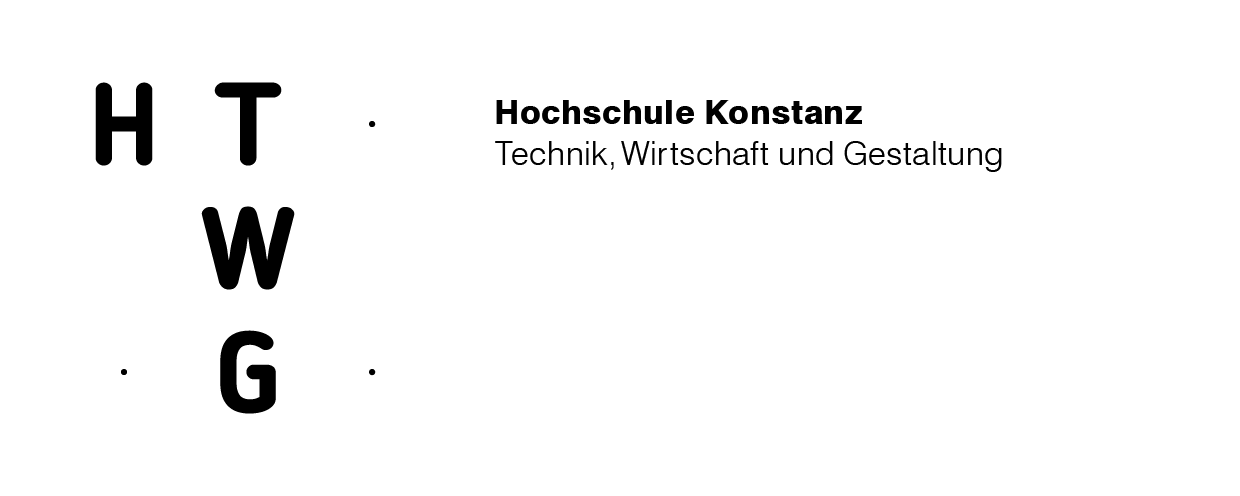
\includegraphics[width=15.7cm]{preface/htwg-logo}
\end{flushleft}

\vspace{1cm}

\begin{center}
	\large{
		\textbf{\strLecture} \\[2cm]
	}
	\Huge{
		\textbf{\strTopic} \\[2cm]
	}
	\Large{
		\textbf{\strAuthorA, \strAuthorB}} \\[3cm]
		%\textbf{\strAuthorA, \strAuthorB, \strAuthorC}} \\[3cm]
	\large{
		\textbf{} \\[2.3cm]
	}
	
	\large{
		\textbf{Konstanz, \strDate}
	}
\end{center}

\end{titlepage}
\thispagestyle{empty}




\begin{center}
{\Large \textbf{Zusammenfassung (Abstract)}}
\end{center}

\bigskip

\begin{center}
	\begin{tabular}{p{2.8cm}p{5cm}p{5cm}}
		Thema: & \multicolumn{2}{p{10cm}}{\raggedright\strTopic} \\
		 & & \\
		Autoren: & \strAuthorA & \href{mailto:\strAuthorAEmail}{\strAuthorAEmail} \\
		 & \strAuthorB & \href{mailto:\strAuthorBEmail}{\strAuthorBEmail} \\
%		 & \strAuthorC & \href{mailto:\strAuthorCEmail}{\strAuthorCEmail} \\
		 & & \\
		Betreuer: & Prof. Dr. Matthias O. Franz & \href{mailto:mfranz@htwg-konstanz.de}{mfranz@htwg-konstanz.de} \\
		 &  Jürgen Keppler & \href{mailto:juergen.keppler@htwg-konstanz.de}{juergen.keppler@htwg-konstanz.de} \\
		 &  Mert Zeybek & \href{mailto:me431zey@htwg-konstanz.de}{me431zey@htwg-konstanz.de} \\
	\end{tabular}
\end{center}

\bigskip

\noindent
\strAbstract

\thispagestyle{preface}



\clearpage

%
% TABLE OF CONTENTS
%
\pagestyle{preface}
%
% TABLE OF CONTENTS
%
\tableofcontents
\newpage


%
% Abbildungsverzeichnis
%
%
% Abbildungsverzeichnis
%
\phantomsection
\addcontentsline{toc}{chapter}{Abbildungsverzeichnis}
\listoffigures
\thispagestyle{preface}
\newpage
\clearpage

%
% Tabellenverzeichnis
%
%
% Tabellenverzeichnis
%
\phantomsection
\addcontentsline{toc}{chapter}{Tabellenverzeichnis}
\listoftables
\thispagestyle{preface}
\newpage
\clearpage



%--------------------------
% ╔═╗╦  ╦╔═╗╔═╗╔╦╗╔═╗╦═╗╔═╗ 
% ║    ╠═╣╠═╣╠═╝  ║   ║╣  ╠╦╝╚═╗ 
% ╚═╝╩  ╩╩  ╩╩      ╩   ╚═╝╩╚═╚═╝ 
%--------------------------

\pagenumbering{arabic} 
\setcounter{page}{1} 
\pagestyle{default}

%
% CHAPTER Versuch 1
%
\chapter{Aufnahme und Analyse eines Grauwertkeiles}

\section{Fragestellung, Messprinzip, Aufbau, Messmittel}
\label{chap:VERSUCH_1_FRAGESTELLUNG}
Ein Python Skript schreiben (s. Anhang A.1.1), welches das Objekt mithilfe der OpenCV aufnehmen. Die Position und die Distanz zwischen der Digitalkamera (in diesem Fall Webcam) und das Grauwertkeil so einzustellen, dass sich die möglichst kompletten Grauwertverlauf in das Bild befindet. Dabei sollte die Grauwertstufen parallel zu den Bildrändern verlaufen.
Mit OpenCV die Belichtungsparameter einzustellen, so dass den weißen Bereich des Bildes keinen Überlauf hat (255 nicht überschreiten), da die Informationen beim Überlauf verloren gehen. Diese Einstellung (Distanz und Belichtungsparameter) benutzt man für alle durchzuführende Versuche. Das aufgenommene Bild(Farbbild) in ein Grauwertbild mit cv2.cvtColor() umwandeln. 
Der Grauwertverlauf in 5 Grauwertstufe aufteilen und als eigene Bilder speichern. Von jeder Grauwertstufe sind der Mittelwert und Standardabweichung zu ermitteln.(s. Anhang A.1.2)
\begin{figure}[H]
	\centering\small
	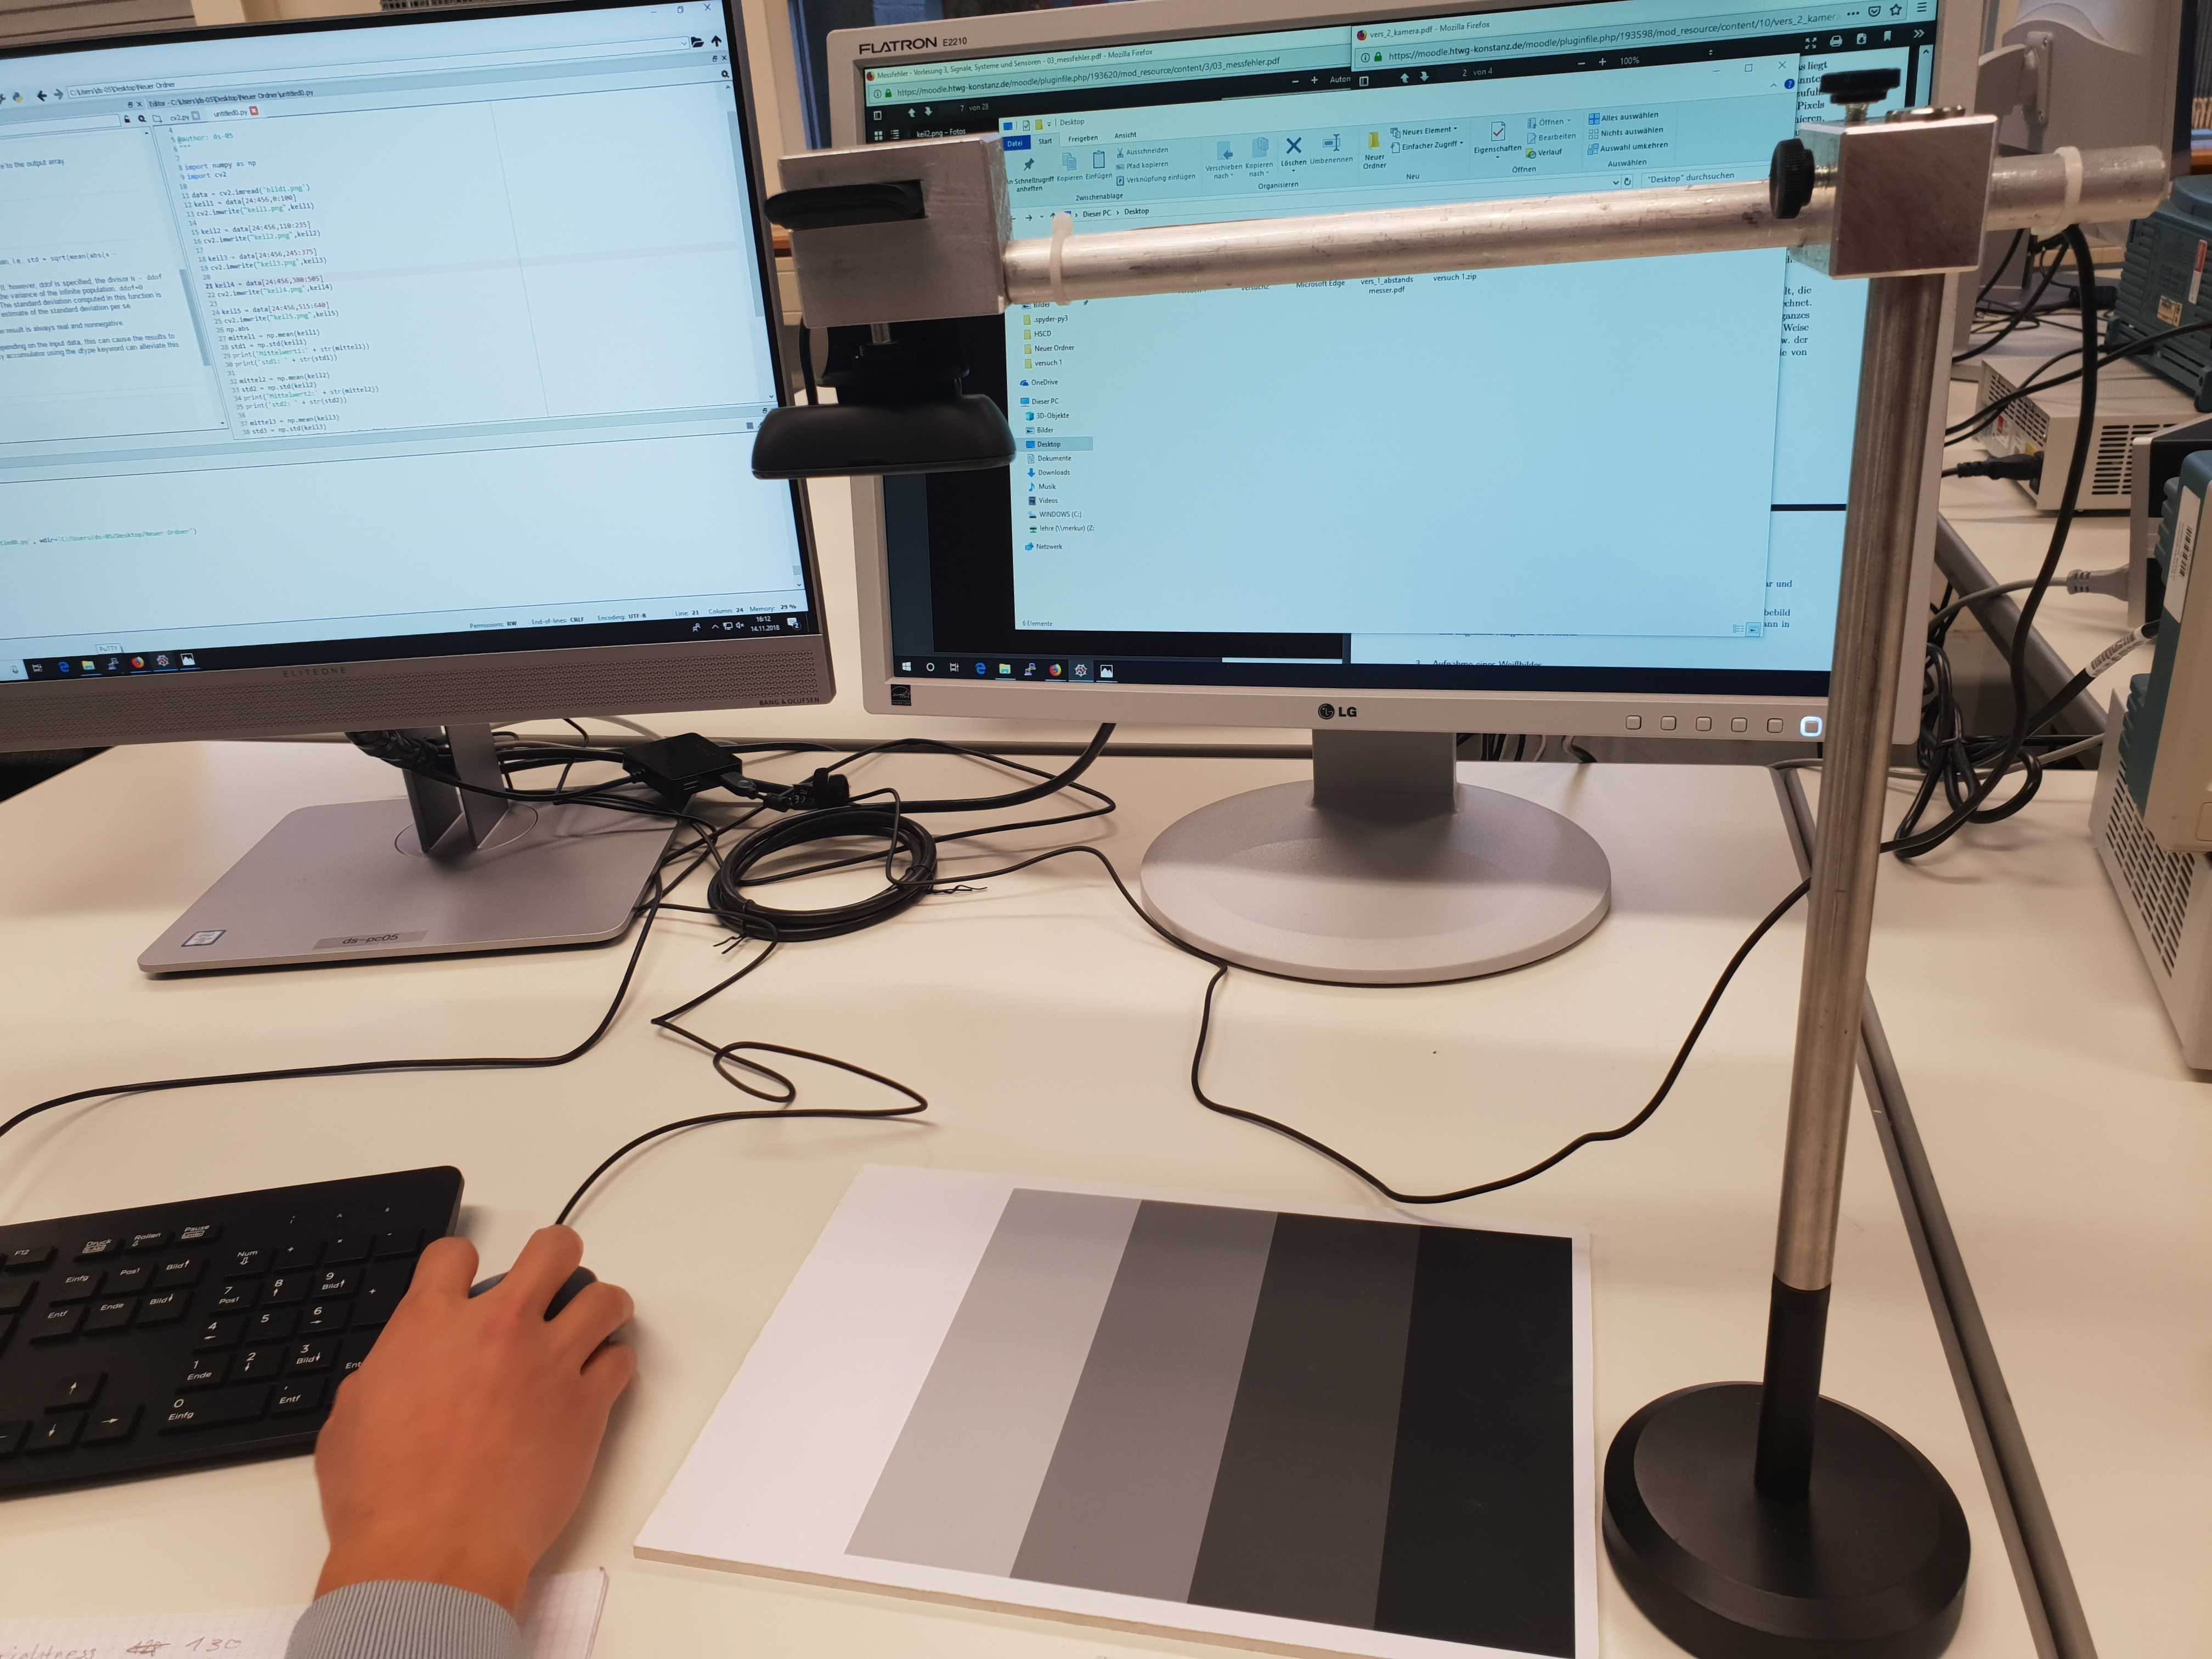
\includegraphics[width=11cm]{versuch_aufbau.jpg}
	\caption{Versuchaufbau}
\end{figure}
\begin{table}[H]
\centering
\begin{tabular}{|l|l|}
\hline
\multicolumn
{1}{|c|}{Belichtungsparameter}	& \multicolumn{1}{c|}{}		\\ \hline
framewidth						&$640$					\\ \hline
frameheight						&$480$					\\ \hline
brightness						&$130$					\\ \hline
contrast						&$30$					\\ \hline
saturation						&$64$					\\ \hline
gain							&$0$					\\ \hline
exposure						&$-4$					\\ \hline
white balance					&$4980$				\\ \hline
\end{tabular}
\caption{Kameraeinstellung}
\end{table}
\section{Messwerte}
\label{chap:VERSUCH_1_MESSWERTE}
\begin{figure}[H]
	\centering\small
	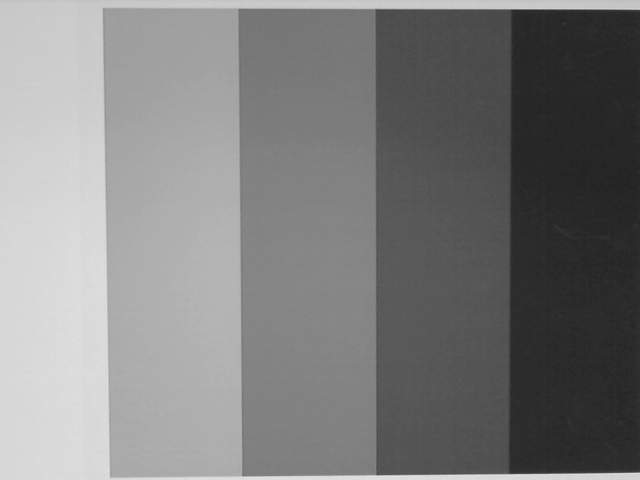
\includegraphics[width=11cm]{bild1.png}
	\caption{Das umgewandelte Grauwertkeilbild}
\end{figure}
\section{Auswertung}
\label{chap:VERSUCH_1_AUSWERTUNG}
Den Code für die Aufteilung und Berechnung bitte den Anhang A.1.2 sehen.\\
\textit{Mittelwert: }	$$\bar{x} = \frac{1}{n}\sum_{i=1}^nx_i$$
\textit{Standardabweichung: }$$s=\sqrt{\frac{1}{n-1}\sum_{i=1}^n{(\bar{x}-x_i)}^2}$$
\begin{table}[H]
\centering
\begin{tabular}{|l|l|l|}
\hline
\multicolumn{1}{|c|}{} & \multicolumn{1}{c|}{Mittelwert} & \multicolumn{1}{c|}{Standardabweichung}\\ \hline
Grauwertstufe 1						&$212.504769$		&$5.643870$					\\ \hline
Grauwertstufe 2						&$170.716981$		&$6.199961$					\\ \hline
Grauwertstufe 3						&$128.680235$		&$4.864795$					\\ \hline
Grauwertstufe 4						&$83.420426$		&$4.632894$					\\ \hline
Grauwertstufe 5						&$41.393944$		&$2.515164$					\\ \hline
\end{tabular}
\caption{Mittelwert und Standardabweichung von Grauwertstufen (Grauwertstufe 1 die hellste bis Grauwertstufe 5 die dunkelste)}
\end{table}

\section{Interpretation}
\label{chap:VERSUCH_1_INTERPRETATION}
Das OpenCV-Paket liest das Bild als Rot-Grün-Blau-Werte(RGB) von jedem Pixel unter eine Matrix ein, deswegen umso dunkler das Keil ist, umso geringer sind die Werte(d.h. (0,0,0) ist komplett schwarz bzw. (255,255,255) komplett weiß) und da das Farbbild in Graubild umgewandelt wurde sind die RGB-Werte jedes Pixels immer gleich. Es folgt darauf, dass die Mittelwerte absteigen, je nach der Helligkeit der Stufen.

Aus den berechneten Standardabweichungen kann man interpretieren, dass die mit größeren RGB-Werten Grauwertstufe mehr variieren als die mit kleineren. 
Bei Grauwertstufe 1 haben wir kleineres Unterbild(weniger Pixel) als anderen Stufe, deshalb zu kleinere Standardabweichung führt.  Die dunklere Grauwertstufen haben auch kleineren Standardabweichung, weil der Unterschied von kleineren Wert kleiner sind als größeren Wert.
%
% CHAPTER Versuch 2
%
\chapter{Aufnahme eines Dunkelbildes}
\section{Fragestellung, Messprinzip, Aufbau, Messmittel}
Um das Schwarzbild aufzunehmen, sollte das Objektiv der Kamera abgedeckt werden, sodass das Bild komplett schwarz wird. Die Belichtungsparameter und Distanz sind gleich wie das erste Versuch einzustellen.

Um das thermische Ausleserauschen zu eliminieren, werden 10 Bilder aufgenommen und daraus berechnet ein pixelweisen Mittelwert(ein ganzes Bild von Mittelwert). Es bleibt nur noch der Offset. bzw der Dunkelstrom jedes Pixels übrig. Das Mittelwertbild ist das Dunkelbild.

Das Eingabebild wird durch Subtraktion von Dunkelbild korrigiert.
\section{Messwerte}
\label{chap:VERSUCH_2_MESSWERTE}
\begin{figure}[H]
	\centering\small
	
\includegraphics[width=11cm]{bildschwarz1.png}
	\caption{Ein aufgenommenes Beispielschwarzbild}
\end{figure}
\begin{figure}[H]
	\centering\small
	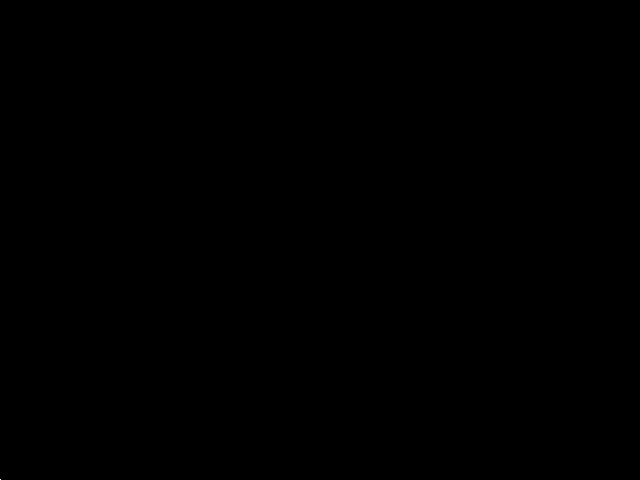
\includegraphics[width=11cm]{kontrastmaxBlack.png}
	\caption{Kontrastmaximierte Darstellung des Dunkelbildes}
\end{figure}
\section{Auswertung}

\label{chap:VERSUCH_2_AUSWERTUNG}
Um das kontramaximierte Bild darzustellen, verwendet man diese Formel für jeden Pixel:
	$$\frac{pixel - min}{max-min}\cdot255$$
	min ist der minimalwert des Arrays/Bildes, max der maximale.
	
Das Dunkelbild mit einem Pythonskript einlesen, von dem Eingabebild subtrahiert und bekommt man das Bild:
\begin{figure}[H]
	\centering\small
	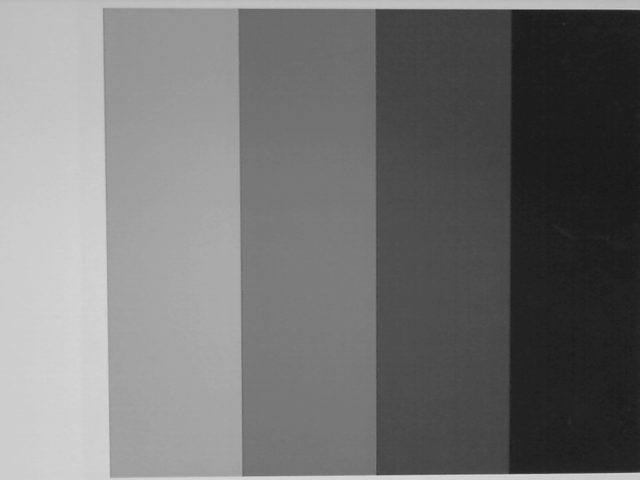
\includegraphics[width=11cm]{korrigiertesBildv2.png}
	\caption{Korrigiertes Eingabebild nach dem Subtrahieren}
\end{figure}

Den Code davon bitte den Anhang A.1.3 sehen.
\section{Interpretation}
\label{chap:VERSUCH_2_INTERPRETATION}
Das berechnete Dunkelbild hat die Werte ungefähr 10 d.h. dass der Offset der von Fertigungstoleranzen und Wärmezufuhr entsteht beträgt 10. Da das Eingabebild von Dunkelbild abgezogen wurde, sieht das korrigierte Bild dunkler aus.
%
% CHAPTER Versuch 3
%
\chapter{Aufnahme eines Weißbildes}


\section{Fragestellung, Messprinzip, Aufbau, Messmittel}
Ein leeres weißes Blatt Papier unter dieselbe Bedingungen wie vorherige Versuche einstellen und 10 Weißbilder aufnehmen zur Elimination des thermischen Rauschens,
das Mittelwertbild wie vorher berechnen. Danach muss man noch das Dunkelbild von dem Mittelwertbild subtrahieren.
Das resultierende Weißbild sollte normiert werden, sodass sein Mittelwert 1 ist, damit das Eingangbild durch Dividieren weiter korrigiert werden könnte. 
\section{Messwerte}
\label{chap:VERSUCH_3_MESSWERTE}
\begin{figure}[H]
\centering\small
\fbox{
	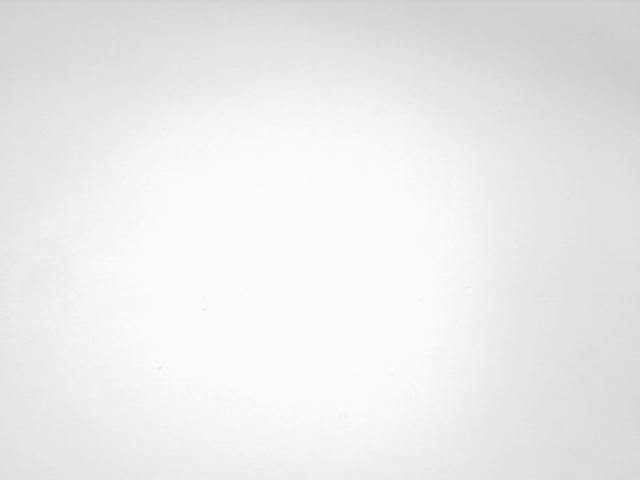
\includegraphics[width=11cm]{bildweiss1.png}
	}
	\caption{Ein aufgenommenes Beispielweißbild}
\end{figure}
\begin{figure}[H]
\centering\small
\fbox{
	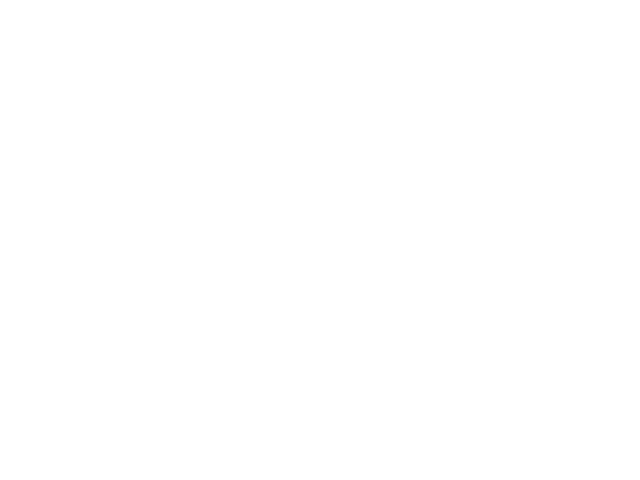
\includegraphics[width=11cm]{kontrastmaxWhite.png}
	}
	\caption{Kontrastmaximierte Darstellung des Weißbildes}
\end{figure}
\section{Auswertung}
\label{chap:VERSUCH_3_AUSWERTUNG}
Um das kontramaximierte Bild darzustellen, verwendet man diese Formel für jeden Pixel:
	$$\frac{pixel}{max-min}\cdot255$$
	min ist der minimalwert des Arrays/Bildes, max der maximale.
	
	Da man die Korrektur mit dem Schwarzbild gemacht hat, ist die Formel anders als die von dem 2. Versuch (pixel - min wird pixel).
	
	Um das Mittelwertbild zu normieren, verwendet man die Formel pixelweise:
	$$normW = \frac{korrigiertes\:Weissbild}{Mittelwert\:von\:dem\:korrigierten\:Weissbild}$$
dadurch bekommt ein neues Bild mit Mittelwert 1.
\begin{figure}[H]
	\centering\small
	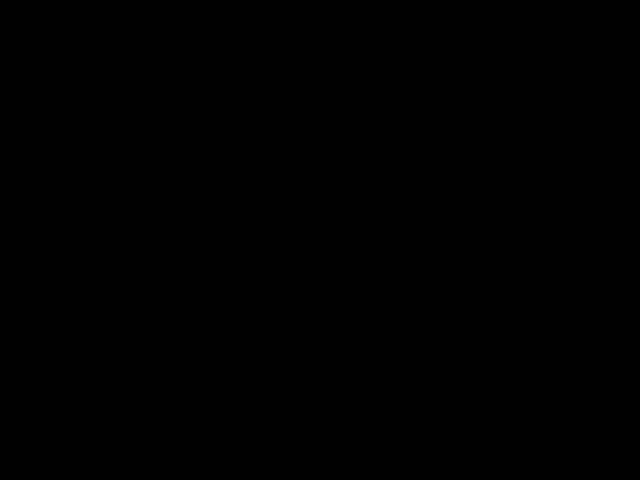
\includegraphics[width=11cm]{normW.png}
	\caption{Normiertes Weißbild}
\end{figure}
Den Code davon bitte den Anhang A.1.3 sehen.
\section{Interpretation}
\label{chap:VERSUCH_3_INTERPRETATION}
Da der Mittelwert von dem normierten Bild 1 ist, sollte das resultierte Bild fast komplett schwarz sein. 

Normalerweise hat das aufgenommene Bild immer eine Vignettierung(dunklere Ränder),die schwer zu erkennen(weil das Objekt eigene Farbwerte besitzt) und aufgrund der unterschiedliche Helligkeitsübertragung von der Optik der Kamera entstand. Mit Weißbild entdeckt man die Vignettierung leichter(weiße Farbe hat größere RGB-Werte -> Unterschied zwischen Ränder und andere Teile des Bildes besser erkennen).
% CHAPTER Versuch 4
%
\chapter{Pixelfehler}
\label{chap:VERSUCH_4}

\section{Fragestellung, Messprinzip, Aufbau, Messmittel}
\label{chap:VERSUCH_4_FRAGESTELLUNG}
Dunkelbild auf dem Bildschirm auf stuck und hot pixels und  Weißbild auf dead pixels überprüfen.
Das Bild des Grauwertkeils mit gleicher Methode im Versuch 3 korrigieren. Korrigiertes Bild in 5 Stufen wie im Versuch 1 aufteilen und überprüft ob es da Verbesserung gibt.

\section{Messwerte}
\label{chap:VERSUCH_4_MESSWERTE}
\begin{figure}[H]
	\centering\small
	
\includegraphics[width=11cm]{mBlack.png}
	\caption{Schwarzbild ohne gefundene hot und stuck pixels }
\end{figure}
\begin{figure}[H]
	\centering\small
	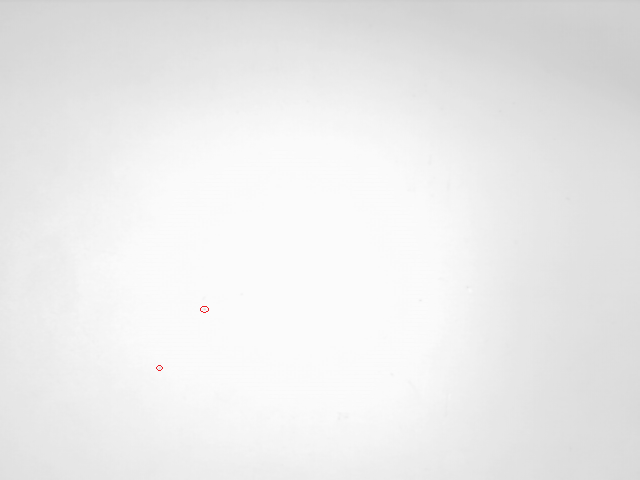
\includegraphics[width=11cm]{mWhitev4.png}
	\caption{Weißbild mit dead pixels Markierung}
\end{figure}
\section{Auswertung}
\label{chap:VERSUCH_4_AUSWERTUNG}
\begin{figure}[H]
	\centering\small
	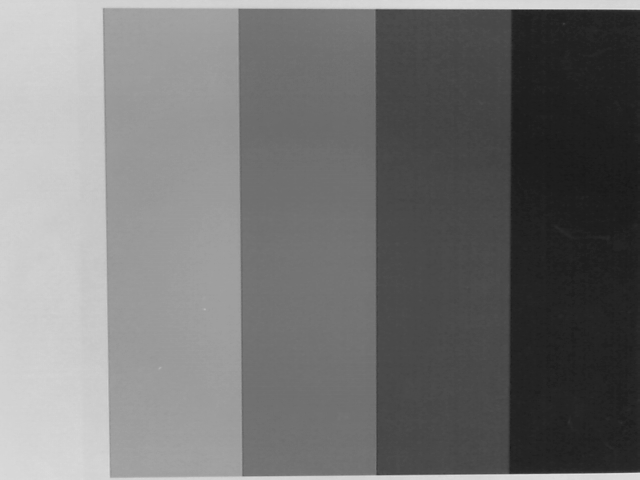
\includegraphics[width=11cm]{Bild1_korrekt.png}
	\caption{Korrigiertes Bild}
\end{figure}
\begin{table}[H]
\centering
\begin{tabular}{|l|l|l|}
\hline
\multicolumn{1}{|c|}{} & \multicolumn{1}{c|}{Mittelwert} & \multicolumn{1}{c|}{Standardabweichung}\\ \hline
Grauwertstufe 1						&$205.782106$		&$3.502565$					\\ \hline
Grauwertstufe 2						&$155.267629$		&$2.611407$					\\ \hline
Grauwertstufe 3						&$113.188105$		&$2.333321$					\\ \hline
Grauwertstufe 4						&$72.236704$		&$2.395081$					\\ \hline
Grauwertstufe 5						&$33.400926$		&$2.649814$					\\ \hline
\end{tabular}
\caption{Mittelwert und Standardabweichung von Grauwertstufen (Grauwertstufe 1 die hellste bis Grauwertstufe 5 die dunkelste)}
\end{table}

\section{Interpretation}
\label{chap:VERSUCH_4_INTERPRETATION}
Bei der Markierung der hot und stuck pixels konnten gar keine Weißpunkte mit normalen Augen entdeckt werden. Das könnte bedeuten, dass die Qualität des Bildsensors noch in guten Zustand ist.

Bei der Markierung der dead pixels sieht man 2 kleine Dunkelbereiche, von der wir behaupten können, dass es nicht nur aus dem Sensor kommt sondern auch wegen der Oberfläche von dem Objekt(nicht ganz homogene Fläche).

Das korrigierte Bild ist dunkler geworden(da Mittelwert geringer ist). Die geringere Standardabweichung weist darauf hin, dass die Unterschied zwischen Pixels in jeder Grauwertstufe kleiner wird. D.h. wir haben eine bessere Bildqualität bekommen.
%
% CHAPTER Anhang
%
\renewcommand\thesection{A.\arabic{section}}
\renewcommand\thesubsection{\thesection.\arabic{subsection}}

\chapter*{Anhang}
\label{chap:APPENDIX}
\addcontentsline{toc}{chapter}{Anhang}
%\setcounter{chapter}{0}
\addtocounter{chapter}{1}
\setcounter{section}{0}

\section{Quellcode}
\label{chap:APPENDIX_SOURCECODE}

\subsection{Quellcode Bild aufnehmen}
\label{chap:APPENDIX_SOURCECODE_V1}
\begin{lstlisting}[
style=PYTHON,
frame=single,
caption=,
captionpos=b,
label=lst:V1]
import numpy as np
import cv2

cap = cv2.VideoCapture(0)
cap.set(11,30)
cap.set(10,130)
cap.set(14,0)
cap.set(15,-4)
cap.set(17,4980)

print("framewidth:" + str(cap.get(3)))
print("frameheight:" + str(cap.get(4)))
print("--------------------------------")
print("brightness:" + str(cap.get(10)))
print("contrast:" + str(cap.get(11)))
print("saturation:" + str(cap.get(12)))
print("--------------------------------")
print("gain:" + str(cap.get(14)))
print("exposure:" + str(cap.get(15)))
print("--------------------------------")
print("white_balance:" + str(cap.get(17)))


while(True):
    ret, frame = cap.read()
    gray = cv2.cvtColor(frame, cv2.COLOR_BGR2GRAY)
    cv2.imshow('frame', gray)
    if cv2.waitKey(1) & 0xFF == ord('q'):
        cv2.imwrite('bildweiß10.png',gray)
        print(np.min(gray),np.max(gray))
        break;
        
cap.release()
cv2.destroyAllWindows()
\end{lstlisting}

\subsection{Quellcode für Bildunterteilung und der Berechnung von Mittelwert und Standardabweichung}
\label{chap:APPENDIX_SOURCECODE_V2}
\begin{lstlisting}[
style=PYTHON,
frame=single,
caption=,
captionpos=b,
label=lst:V2]
import numpy as np
import cv2

data = cv2.imread('bild1.png')
print(data)
keil1 = data[24:456,0:100]
cv2.imwrite("keil1.png",keil1)

keil2 = data[24:456,110:235]
cv2.imwrite("keil2.png",keil2)

keil3 = data[24:456,245:375]
cv2.imwrite("keil3.png",keil3)

keil4 = data[24:456,380:505]
cv2.imwrite("keil4.png",keil4)

keil5 = data[24:456,515:640]
cv2.imwrite("keil5.png",keil5)

data = cv2.imread('bild1_korrekt.png')
keil1_k = data[24:456,0:100]
cv2.imwrite("keil1_korrekt.png",keil1_k)

keil2_k = data[24:456,110:235]
cv2.imwrite("keil2_korrekt.png",keil2_k)

keil3_k = data[24:456,245:375]
cv2.imwrite("keil3_korrekt.png",keil3_k)

keil4_k = data[24:456,380:505]
cv2.imwrite("keil4_korrekt.png",keil4_k)

keil5_k = data[24:456,515:640]
cv2.imwrite("keil5_korrekt.png",keil5_k)

def MuS(keil, n):
    mittel = np.mean(keil)
    std = np.std(keil)
    print('Mittelwert'+ str(n) +':' + str(mittel))
    print('std'+ str(n) +':' + str(std))
MuS(keil1, 1)
MuS(keil2, 2)
MuS(keil3, 3)
MuS(keil4, 4)
MuS(keil5, 5)
print('korrigierte Werte:--------------------------------------')
MuS(keil1_k, 1)
MuS(keil2_k, 2)
MuS(keil3_k, 3)
MuS(keil4_k, 4)
MuS(keil5_k, 5)
\end{lstlisting}

\subsection{Quellcode zum Einlesen, Auslesen, Korrigieren des Eingangbild mithilfe des Weiß-und Schwarzbildes}
\label{chap:APPENDIX_SOURCECODE_V3}
\begin{lstlisting}[
style=PYTHON,
frame=single,
caption=,
captionpos=b,
label=lst:V2]
import numpy as np
import cv2

bild1 = cv2.imread('bild1.png')

def mw(bild): #Bildern einlesen und Mittelwert für jede Pixel bilden
    data = []
    datad = []
    for i in range(1,11):
        data.append(cv2.imread(str(bild) + str(i) + '.png'))
    for i in data:
        datad.append(i.astype(float))
    mw = np.zeros(datad[0].shape)
    for i in range(0,480):
        for j in range(0,640):
            for k in range(0,10):
                mw[i,j] += datad[k][i,j]
    for i in range(0,480):
        for j in range(0,640):
            mw[i,j] /= 10
    return mw
    
def konmaxb(pixel):
    return ((pixel - np.min(pixel)) / (np.max(pixel) - np.min(pixel))) * 255

def konmax(pixel):
    return (pixel / (np.max(pixel) - np.min(pixel))) * 255

mwb = mw('bildschwarz') #Mittelwert von Dunkelbildern
cv2.imwrite("mBlack.png", mwb)
cv2.imwrite("kontrastmaxBlack.png", konmaxb(mwb)) #Ausgabe kontrastmaximiertes Dunkelbildes

korBv2 = bild1 - mwb
cv2.imwrite("korrigiertes Bild v2.png", korBv2)

mww = mw('bildweiss') #Mittelwert von Weißbildern
cv2.imwrite("mWhite.png", mww)
cv2.imwrite("kontrastmaxWhite.png", konmax(mww-mwb)) #Ausgabe kontrastmaximiertes Weißbildes
normW = (mww-mwb)/np.mean(mww-mwb) # nomiertes Weißbild
cv2.imwrite("normW.png", normW)
korW = korBv2 / normW
cv2.imwrite("Bild1_korrekt.png", korW)
\end{lstlisting}

\end{document}
%------------------------------------
% ╔═╗╔╗╔╔╦╗  ╔╦╗╔═╗╔═╗╦  ╦╔╦╗╔═╗╔╗╔╔╦╗
% ║╣  ║║║  ║║     ║║║  ║║    ║  ║║║║║ ╣  ║║║ ║ 
% ╚═╝╝╚╝═╩╝  ═╩╝╚═╝╚═╝╚═╝╩  ╩╚═╝╝╚╝  ╩ 
%------------------------------------